\documentclass[10pt,twocolumn,letterpaper]{article}
%% Welcome to Overleaf!
%% If this is your first time using LaTeX, it might be worth going through this brief presentation:
%% https://www.overleaf.com/latex/learn/free-online-introduction-to-latex-part-1

%% Researchers have been using LaTeX for decades to typeset their papers, producing beautiful, crisp documents in the process. By learning LaTeX, you are effectively following in their footsteps, and learning a highly valuable skill!

%% The \usepackage commands below can be thought of as analogous to importing libraries into Python, for instance. We've pre-formatted this for you, so you can skip right ahead to the title below.

%% Language and font encodings
\usepackage[english]{babel}
\usepackage[utf8x]{inputenc}
\usepackage[T1]{fontenc}

%% Sets page size and margins
\usepackage[a4paper,top=3cm,bottom=2cm,left=3cm,right=3cm,marginparwidth=2cm]{geometry}

%% Useful packages
\usepackage{amsmath}
\usepackage{graphicx}
\usepackage{appendix}
\usepackage{pdflscape}
\usepackage[colorinlistoftodos]{todonotes}
\usepackage[colorlinks=true, allcolors=blue, breaklinks]{hyperref}
\usepackage[numbers]{natbib}
\bibliographystyle{IEEEtranN}

%% Title
\title{
        \usefont{OT1}{bch}{b}{n}
        \normalfont \normalsize \textsc{UFSC 2023 - Embedded Systems Programming in C++} \\ [10pt]
        \huge Helmholtz Cage Driver \\
}
\selectlanguage{english}
\usepackage{authblk}
\author[1]{Ramon de Araujo Borba}
\affil[1]{UFSC - Universidade Federal de Santa Catarina}

\begin{document}
\maketitle

\iffalse
\begin{abstract}

\end{abstract}

{\textbf{Keywords} \newline
Embedded Systems, Helmholtz Cage, OOP, C++}
\fi

\section{Introduction}

The Helmholtz cage is composed of a set of coils, positioned concentrically along three orthogonal axis. By controlling the current flowing through the coisl, it is possible to genereate a uniform magnetig field in the center of the cage, in any desired direction.

Some of the applications of this equiment includes adjustment and calibration of magnetic sensors, testing of electronic devices, development and environmental simulations for nanosatellites, academic researches, scientific experiments and more.

In the Drakkar Atlantec Group calibration laboratory, a Helmholtz cage is used for adjustment and calibration of oceanography equipments, which includes magnetic sensors.
It was observed by one of the owners of this company that the driver and software used in their laboratory for controlling their Helmholtz cage is becoming obsolete, and maintenance and repair of this driver is of great difficulty.

In this context, this work presents the design and implementation of a Helmholtz cage driver, capable of controlling Helmholtz coils in 3 axis, and adequate for use in the calibration laboratory of the Drakkar Atlantec Group.

The development of this project is part of the course EEL510265 - Embedded Systems Programming, the complete project requirements provided by professor Eduardo Augusto Bezerra can be found in his website\cite{projspecs} and in the project's GitHub repository's\cite{mygit} Documentation Folder.

\section{Application Requirements}

For adequate use in the Drakkar Atlantec laboratory, the embedded controller must fulfill the following requirements:
\begin{itemize}
  \item Provide currents of up to $1.5 A$ in both directions to the coils of each axis.
  % \item \textcolor{red}{resolution requirements?}
  \item Have current monitoring capability.
  % \item \textcolor{red}{resolution requirements?}
  \item Allow control of the axes via serial communication with a host computer.
  % \item \textcolor{red}{anything else?}
\end{itemize}

Besides the requirements for laboratory use, this controller will have the following features:
\begin{itemize}
  % \item \textcolor{red}{Any requirements from prof. Bezerra that are not mentioned above}
  \item Control and monitoring via wireless communication with a host smartphone.
  \item Store a log of operations and events.
\end{itemize}

The host computer and smartphone software have the following requirements:
\begin{itemize}
  \item Allow user to control each axis individually.
  \item Read the event log from the embedded system.
  \item Allow user to visualize the log of events:
  \begin{itemize}
    \item List all events between a given time interval.
    \item Checking total active time of the embedded system between a given time interval.
  \end{itemize}
\end{itemize}

\section{Materials \& Methods}

The hardware for the embedded system will be comprised of a processing unit, voltage controlled current sources, helmholtz coils, current sensors and a real time clock.

The chosen processing unit is an ESP32 based development kit featuring the ESP32-WROOM-32\cite{esp32} dual-core microcontroller module, with built-in Wi-Fi and Bluetooth capabilities, developed by Espressif \cite{espressif}

The current sources were designed using operational apmlifiers and power transistors, and the ESP32 module controlls the current sources using its internal DAC or PWM signals.
The current sources are designed to provide currents of up to \( \pm 1.5 A \).

The current sensors are based on INA219 \cite{ina219} and ACS712 \cite{acs712} ICs. The INA219 current sensor has a resolution of $0.8 mA$ and the ACS712 current sensor has a sensibility of $66 mV/A$.

The software for the entire system, embedded controller, host computer and host smartphone were developed using C++ with object oriented design.

For the embedded controller, the software was developed using Espressif's ESP-IDF \cite{espidf} framework, which is composed of libraries and drivers for the microcontroller, made by the manufacturer.

\section{Proposed design}

The proposed system is composed of two parts, an embedded controller, for which both hardware and firmware were designed and implemented, and a host computer and smartphone software to interact with the embedded controller. A block diagram for the system is shown in \autoref{fig:sys-block-diagram}.

\begin{figure}[htb]
  \centering
  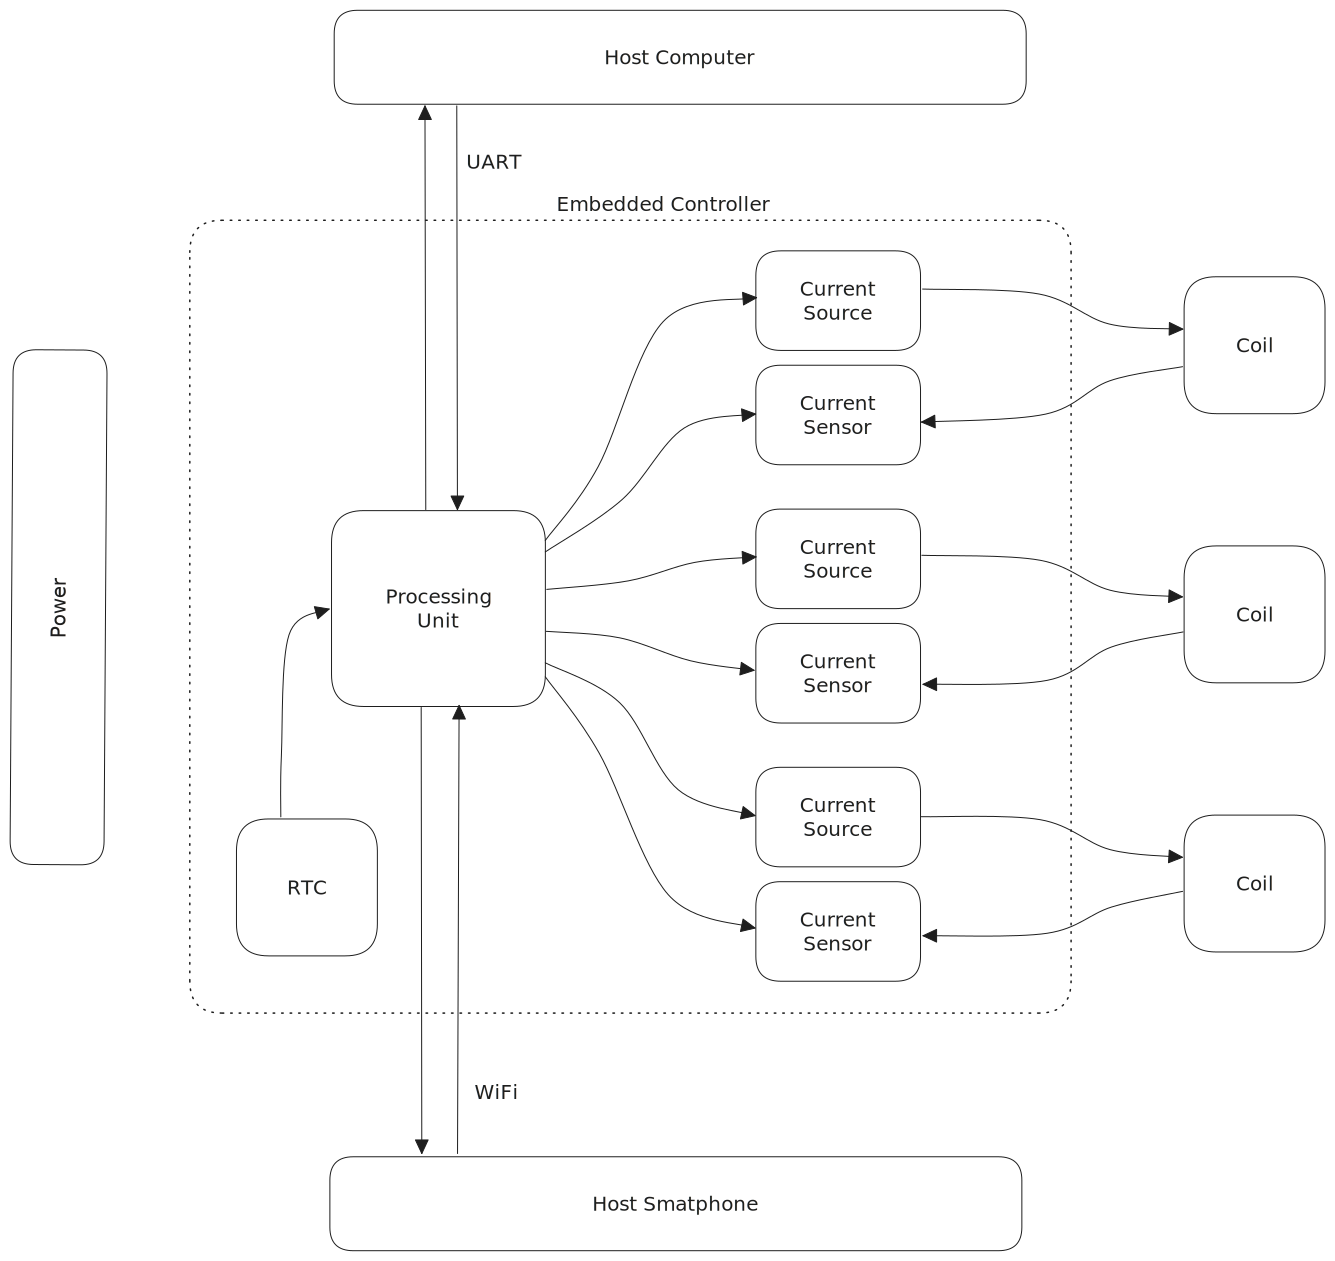
\includegraphics[width=\linewidth, keepaspectratio]{figures/block-diagram.png}
  \caption{System block diagram}
  \label{fig:sys-block-diagram}
\end{figure}

In the sections below, the different parts of the system are explained in more detail.

\subsection{Embedded Hardware}

The embedded controller is composed of a processing unit, three current sources, three current sensors and a real-time clock.

The processing unit chosen was an ESP32 based module \cite{esp32}, which has a dual-core 32-bit microcontroller with a clock frequency of up to $240 MHz$, built-in Wi-Fi and Bluetooth capability, 4Mb of Flash memory and a wide variety of  peripherals and sensors.

Due to limited availability, two types of current sensors were used, one INA219\cite{ina219} based current sensor and two ASC712 \cite{acs712} based current sensors.
The INA219 current sensor can measure currents of up to $\pm 3.2 A$ with a resolution of $0.8 mA$, provides digital output through an I\textsuperscript{2}C interface.
The ACS712 current sensor can measure currents of up to $\pm 30 A$ with a sensibility of $66 mV/A$ and porvides analog output, requiring the use of an ADC.

The real-time clock module is based on the DS3231 \cite{ds3231} chip, which has an integrated temperature compensated oscilator crystal for increased accuracy, integrated temperature sensor and programmable square wave output signal.

The voltage controlled current sources were designed using LM324 \cite{lm324n} operatoinal amplifiers and TIP41 and TIP42 \cite{tip4x} power transistors.
The current sources are designed to provide currents of up to $\pm 1.5 A$ and can be controlled by a voltage signal.
The EPS32 has two integrated 8-bit DAC channels that are used to control two af the three current sources, the remaining one is controlled through a PWM output filtered by an passive RC filter.
The schematic for the current source circuit is shown in \autoref{fig:schm-current-source} of \autoref{app:schematics}.

\subsection{Embedded Firmware}

The firmware for the embedded system was implemented using the Espressif's ESP-IDF\cite{espidf} official development framework and it's available tools.
This framework runs a slightly modified version of FreeRTOS\cite{freertos} natively, and allows the developer to use all of it's features.
The FreeRTOS was modified by Espressif in order to allow it perform in ESP32's dual-core architecture, and manage both cores effectively, allowing for multithreaded development.
Due to that, the embedded firmware was designed with the FreeRTOS workflow in mind, mainly through the use of tasks, to accomplish its goals.
Details about the modifications can be found in the ESP-IDF Programming Guide\cite{espidf}.

Although the ESP-IDF framework's features and APIs being implemented in C, it is natively compatible with C++ development, due to the compilers being built upon GCC, it even provides example components and APIs implemented in C++ which are used in this application where possible.

The firmware must fulfillthe following tasks:
\begin{itemize}
  \item Host computer communication via UART.
  \item Host smartphone communication via Wi-Fi/Bluetooth.
  \item Control each Helmholtz coil idependently through PWM or DAC.
  \item Read current sensors for each Helmholtz coil.
  \item Record a log of events.
  \item Transfer the event log to the hosts.
\end{itemize}

\subsubsection{Abstraction Layers}

The firmware will be organized in layers with different levels of abstraction. The highes layer will be responsible for the application logic and operation, with lower layers being responsible for external devices and basic functions of the microcontroller and its peripherals, astracting the manufacturer's C labraries using C++ classes.

The abstraction layers are divided as follows:
\begin{itemize}
  \item Application layer.
  \item Components layer.
  \item Device Drivers layer.
  \item MCU Drivers layes.
\end{itemize}

The MCU Drivers layer is composed of classes responsible for interfacing with the ESP32's internal peripherals and functionalities.
In this layer, most of the ESP-IDF's C APIs are encapsulated into C++ classes and, where possible, the ESP-IDF's own C++ APIs are employed.

The Device Drivers layer is composed of classes responsible for implementing drivers for the external devices used in the system, such as current sensors, current sources and real time clock, taking advantage of the abstractions of the internal drivers of the ESP32.

The Components layer is composed of classes responsible for implementing the interface between the application logic and the hardware devices.
They provide the main functionalities needed by the application.

The Application layer, which is mainly composed of the Application class, is the highes level layes and is responsible for the logic of operation of the embedded controller and creation of the main application task.

\subsubsection{Detailed Description}

In order to fulfill the requirements for this application, and following the abstraction layers described above, several C++ classes were designed.
This section porvides a basic description of each of the main classes responsible for the application logic.
The class diagram for the embedded firmware is shown in \autoref{fig:emb-class-diagram} of \autoref{app:class-diagrams}.

The Application class represents the application as a hole and deals with the application logic, it is the entry point of the system firmware.
This class is responsible for creating the main tasks of the system, and integrating the othe component classes to control the system's operation.

The Host, HostPC and HostMobile classes represent the hosts of the system, which will receive the log of events and send commands to de embedded controller.
The Host class is an abstract class, providing methods for the Application class to interface with all of its hosts through polymorphism and virtual functions.
The HostPC class inherits from the Host class and represents the host PC, which will be interfaced with via UART.
The HostMobile class also inherits from the Host class and represents the host PC, which will be interfaced with via WiFi.
Both hosts will be able to send commands for controlling the current sources individually, as well as request the transmisison of the log of events.

The Queue and Node template classes implemet a queue data structure.
They are designed to be platform independant, flexible and reuseble to store any type of object as necessary.
In the embedded controller, the main use for this templated classes is to implmement the log of events.

The Logger and LogData classes represent the system log of events.
The LogData encapsulates all the information needed in a log entry, while the Logger class manages the storage of this information in a queue, to later be sent to the hosts.

The ClockCalendar class is responsible for storing the date and time of each entry in the event log, it inherits from both the Clock and the Calendar classes, which are responsible for dealing with time and dalendar dates respectively.

\subsection{Host computer software}

The host computer software was developed in C++ with an object oriented approach.

It was developed using G++13 compiler, with C++23 standard.

WSL was used to develop the software and for now it only supports Linux.
It is being implemented as platform independant as possible, with portability in mind.
This way, if it is to be used in a different platform, only a small amount od change will be needed.

\subsubsection{Abstraction Layers}

The host computer software is organized in a similar manner as the embedded firmware, with abstraction layers, except it has less layer since its not dealing directly with hardware.

The abstraction layers are divided as follows:
\begin{itemize}
  \item Application layer.
  \item Libraries layer.
\end{itemize}

The application layer is where the logic of operation is implemented, being the highest level of abstraction in the software. It's mainly composed of a Application class.

The libraries layer is composed of several classes, organized as differen libraries, that implement specific functionalities used by the Application class to fulfill the requirements for the software.

\subsubsection{Detailed Description}

In order to fulfill the requirements for this application, and following the abstraction layers described above, several C++ classes were designed.
This section porvides a basic description of each of the main classes responsible for the application logic.

The Application class is te entry point for the program and is responsible for starting the program's threads and sending commands to the embedded controller.

The SerialPort class is responsible for managing serial ports and is used to communicate with the embedded system. Here, an exception is thown to signal if the serial port was successfully opened upon construction of the SerialPort object.

Due to C++'s abstractions mechanisms, some of the classes implemented for the embedded controller were re-used for the host computer software, since they were implmented in a platform agnostic manner.
The Logger, LogData, ClockCalendar, Queue and Node classes were taken from the embedded controller code base, with the only modifications made for adding functionality.

The ability to compare dates throught the ClockCalendar classes was implemented through operator overloading and friends. This functionality was used to compare and select the entries in the event log.


\subsection{Tests}

A test plan was implemented and is present at \autoref{app:test-plan}.

\iffalse

\section{Results}


\section{Discussion}


\section*{Conclusions}

\fi

\bibliography{bibliography}

\onecolumn

\appendix
\appendixpage

\section{Class Diagrams} \label{app:class-diagrams}

\begin{figure}[htb]
  \centering
  \includegraphics[width=\linewidth, keepaspectratio]{figures/emb-class-diagram.png}
  \caption{Embedded firmware class diagram}
  \label{fig:emb-class-diagram}
\end{figure}

\newpage
\section{Schemaitcs \& Simulations} \label{app:schematics}

\begin{figure}[htb]
  \centering
  \includegraphics[width=\linewidth, keepaspectratio]{figures/current-source-schematic.png}'
  \caption{Voltage controlled current source schematic}
  \label{fig:schm-current-source}
\end{figure}

\begin{figure}[htb]
  \centering
  \includegraphics[width=\linewidth, keepaspectratio]{figures/current-source-output.png}'
  \caption{Voltage controlled current source output current simulation}
  \label{fig:sim-current-source-output-current}
\end{figure}


\section{Test Plan} \label{app:test-plan}

\subsection{Required Tools}

To perform the tests described in the next section, the following intruments and software tools are necessary:

\begin{itemize}
  \item Required software tools:
  \begin{itemize}
    \item PC with a Linux OS (Ubuntu preferably)
    \item ESP-IDF v5.1.2
    \item g++ 13.1.0
    \item A terminal emulator (screen or minicom for example)
  \end{itemize}

  \item Required hardware and instruments:
  \begin{itemize}
    \item Voltimeter
    \item Amperimeter
    \item USB/UART converter
    \item ESP32 development board
  \end{itemize}
\end{itemize}

\subsection{HostPC Software Tests}

The following tests verify that the host PC software is operating correctly.

\subsubsection{Test 1}

Verify that the host PC software can send commands through a serial port.

\paragraph{Setup}
\begin{itemize}
  \item Clone the project's GitHub repository \cite{mygit}
  \item Compile the host PC software
  \item Connect the ESP32 to the PC with the appropriate USB cable
  \item Load the uart\_events example from ESP-IDF onto the ESP32
\end{itemize}

\paragraph{Steps}
\begin{itemize}
  \item Open a terminal window and run the ESP-IDF serial monitor on the ESP32 serial port
  \item Execute the host PC software configured for the USB/UART converter serial port
  \item Select option 1 to set the X axis current
  \item Verify on the ESP32's logs that the correct command was sent
  \item Select option 2 to set the Y axis current
  \item Verify on the ESP32's logs that the correct command was sent
  \item Select option 3 to set the Z axis current
  \item Verify on the ESP32's logs that the correct command was sent
  \item Select option 4 to request transmission of the event log from the embedded controller
  \item Verify on the ESP32's logs that the correct command was sent
\end{itemize}

\paragraph{Expected Results}

\begin{itemize}
  \item The correct commands are being sent from the host PC.
\end{itemize}

\subsection{Embedded Controller Tests}

The following tests verify that the embedded controller is operating correctly.

\subsubsection{Test 1}

Verify that the embedded controller can read commands from serial port.

\paragraph{Setup}
\begin{itemize}
  \item Assert that the host PC software tests were executed and the expected results were obtained
  \item Clone the project's GitHub repository \cite{mygit}
  \item Compile the host PC software
  \item Connect the embedded controller to the PC with the appropriate USB cable
  \item Connect the USB/UART converter to the embedded controller's command serial port and the host PC.
  \item Compile and load the firmware of the embedded controller using ESP-IDF's tools
\end{itemize}

\paragraph{Steps}
\begin{itemize}
  \item Open a terminal window and run the ESP-IDF serial monitor on the embedded controller's debug serial port
  \item Execute the host PC software configured for the USB/UART converter serial port
  \item Select option 1 to set the X axis current
  \item Verify on the embedded controller's logs that the correct command was received
  \item Select option 2 to set the Y axis current
  \item Verify on the embedded controller's logs that the correct command was received
  \item Select option 3 to set the Z axis current
  \item Verify on the embedded controller's logs that the correct command was received
  \item Select option 4 to request transmission of the event log from the embedded controller
  \item Verify on the embedded controller's logs that the correct command was received
\end{itemize}

\paragraph{Expected Results}

\begin{itemize}
  \item The correct commands are being received by the embedded controller.
\end{itemize}

\end{document}
